\documentclass[a4paper]{scrartcl}
\usepackage{defaultstyle}
\usepackage{localstyle}

\title{Authorization Logic for Mobile Ecosystems}
\subtitle{Second Year Report}
\author{Joseph Hallett}
\date\today

\begin{document}
\maketitle

\begin{abstract}
  This report describes the second year work of my PhD.
  I give a brief overview of app installation policies and the AppPAL authorisation logic; before describing the work completed this year.
  I review topics suggested in the thesis proposal; and describe my work implementing AppPAL, exploring store and user policies and looking at protocols for app distribution.
  I describe what I expect to work on in the final year of my studies; and finally, I give a table of contents and plan for my producing my thesis in the remaining time available to me.
\end{abstract}

\section{Introduction}

Mobile devices are different to other computers.
They have access to greater personal data than a PC; pictures and photos as well as conversations, locations, and address books.
They mostly run software sold through stores under the manufacturer's control.
People take them to work and on holiday; into their homes and out to the towns and countryside.
These devices communicate through wireless almost exclusively: working with cars via bluetooth, the internet via 3G, speakers TVs and other internet-of-things devices through wifi.
These differences create a different ecosystem for them to operate in: one that we aim to model and control using authorization logic.

Authorization logics are designed to express policies which decide whether a principal, for example a computer user, can perform an action.
They have been used to implement access control systems to decide whether users can read or write to files.
I believe they can also help users decide which apps they want to use.

The interaction between stores, users, apps and phones gives rise to trust relationships between each of the different entities.
Users trust the stores to sell them good, malware-free apps.
Some stores will sell any apps, but others are more picky relying on audits and tools to find the higher quality apps to sell.
In the stores users are told about the apps they might want to buy (\autoref{fig:storeinfo}):
who developed the app, whether they were a \emph{top developer}, what kind of app it is, age ratings, functionality the app may have, aggregated review scores, descriptions and bugs from both anonymous and not so anonymous users, update times, the price of in-app-purchases and the permissions it will request.
How do the device owners know which information to trust?
Where does the store get this information from in the first place?

\begin{figure}\centering
  \includegraphics[width=0.8\linewidth]{images/angrybirds.png}
  \includegraphics[width=0.8\linewidth]{images/reviews.png}
  \includegraphics[width=0.8\linewidth]{images/additionalinfo.png}
  \caption{Information presented to the user in the Play store.}
  \label{fig:storeinfo}
\end{figure}

Finding the right apps can be tricky:
  users need to work out which apps are well written, which are not going to abuse their data, which ones will work in the way they want.
Users and companies need to find the apps which suit how they want to use their devices.
This can be difficult as it isn't obvious how apps use the data they have access to.
There is a large amount of choice.
Apps are picked for a variety of reasons:
  ordering in the store~\citep{Prata:2012in},
  reviews and privacy concerns~\citep{Kelley:2013kc},
  and security rules from employers.
These policies could be written down and used to guide device owners when they are making a decision that goes against them.

For example, one user may wish to only install games that have favourable reviews on their favourite gaming site, and which don't have in-app purchases.
For this user searching a store might be frustrating: they need to work out the permissions of the app, cross reference the apps between the store and the review site.
Using an authorization logic (like AppPAL) we could express the preferences as a policy and by enforcing it only show the user the apps they wanted in the store, or to warn them when they are looking at an app which doesn't meet their policy.
The policy would need to delegate to the review site to decide if the app is good, and to google to decide the category of apps.
We might also need to examine the app itself to decide whether it can make in-app purchases\footnote{On Android the ability to make in-app purchase is controlled through the permissions system.}.
\begin{lstlisting}
`user' says App isInstallable
  if App hasCategory(`game'),
     App isGood
  where hasPermission(App, "IAP") = false.

`user' says `play-store' can-say 0 App hasCategory(Category).
`user' says `review-site' can-say inf App isGood.

`review-site' says App isGood
  where reviewSiteScore(App) > 7.
\end{lstlisting}

If an employer uses a \ac{BYOD} scheme in their company they trust users to follow company IT policies when using their phones at work.
Using tools like Google's \emph{Apps Device Policy}\footnote{\url{https://play.google.com/store/apps/details?id=com.google.android.apps.enterprise.dmagent}} the employer can restrict the use of specific apps.
This is an unsubtle form of control.
We want to block apps by describing the characteristics of the apps we want or do not want.
Blacklisting requires constant updating to keep the list up-to-date.
Blacklisting doesn't allow for rich policies using information from third parties or on the basis of metadata about the app.
There is no scope for making any kind of decision other than to allow an app or not.
For IT departments in these companies these are the only tools to enforce their policies.
For more advanced policies, such as not leaking company documents, compliance is left to employees.

\begin{figure}[]
  \centering
  \includegraphics[width=1.0\linewidth]{images/ecosystem.eps}
  \caption{The mobile ecosystem surrounding a phone used for \ac{BYOD} and the trust relationships surrounding it.}
  \label{fig:ecosystem}
\end{figure}

Policies exist for mobile ecosystems; but there aren't ways of precisely modelling or enforcing them.
Authorization logic could be used to describe these policies and enforce them automatically.
Logics can describe the trust relationships and policies surrounding Android formally.
This lets us make precise statements about the security of these systems.
They can be used to make comparisons between different security models, such as those in iOS and Android.
It allows comparisons between user's privacy policy and their actual behaviour.

By capturing these patterns as policies they can be enforced automatically.
By checking the policies we can enforce them at run-time; or warn when making decisions that go against them.
This reduces the burden on users to decide which apps they want.
Security-savvy users may design policies themselves: these could be shared with others or used in organisation-wide curated app stores.

This thesis research will show how authorization logic can be used to make security decisions in mobile devices.
Currently, security decisions must be made manually by smart phone users.
By automating these choices we believe users can avoid having to make security decisions; improving their overall security.

\subsection{AppPAL}

AppPAL is an instantiation of Becker \etal's SecPAL~\citep{Becker:2006vh} I have developed to model and enforce app installation policies.
Using AppPAL we can describe policies with trust relationships, and which incorporate constraints.
This gives a powerful language to describe user's and company's app policies precisely.

Using AppPAL a principal (someone who utters statements about apps, such as a user or store) can say an app is installable.
\begin{lstlisting}
`user' says `apk://com.rovio.angrybirds' isInstallable.
\end{lstlisting}
Or that an app is installable only \emph{if} some conditions are correct and \emph{where} a constraint is true.
\begin{lstlisting}
`user' says App isInstallable
  if `office-app-policy' isMetBy(App)
  where locationAt(`work') = true.
\end{lstlisting}
There is support for renaming or role assignment.
\begin{lstlisting}
`user' says `ian' can-act-as `it-department'.
\end{lstlisting}
Statements are collected into an \emph{assertion context} which is queried using SecPAL's three evaluation rules~\citep{Becker:2006vh}.

Decisions can be delegated to other principals; with separate versions where further delegation is allowed (\lstinline{inf}) or not (\lstinline{0}).
For example as part of a company policy all apps should come with a statement, from an anti-virus, vendor that the app is not malicious.
To create this relationship the \emph{can-say} statement is used.
For example the company may trust McAfee and Google to decide whether something is malicious or not, but want McAfee to say directly whether an app is malware.
With Google, however, they're happy for them to recommend another anti-virus vendor they trust to make the decision for them.
In the case of McAfee we use \lstinline{can-say 0} and with Google \lstinline{can-say inf}.
\begin{lstlisting}
`company' says `mcafee' can-say 0 App isMalicious.
`company' says `google' can-say inf App isMalicious.
\end{lstlisting}
If, when checking if an app is malicious, we come across a delegation statement from McAfee then it will be ignored.
\begin{lstlisting}
`mcafee' says `f-secure' can-say 0 App isMalicious.
\end{lstlisting}
A delegation from Google, however, could be used to decide whether the app was malicious.
\begin{lstlisting}
`google' says `f-secure' can-say 0 App isMalicious.
\end{lstlisting}

\section{Summary of second year work}

%\subsection{What I said I'd do}

In my thesis proposal I stated I would spend this year looking at the role of app stores.
Specifically I wanted to understand how users interacted with the stores.
This would enable us to better understand their behaviour letting us write policies that accurately described their actions.
I said that I would:
\begin{itemize}
  \item Implement an app store filtered by AppPAL policies.
  \item Look at how users interact with apps, and the kinds of policies they apply, as well as what happens when their policies change.
  \item Look at how the policies vary within categories of apps.
  \item Explore how policies could be composed and joined.
  \item Explore what happens when policies are attacked.
\end{itemize}

These topics changed as the year went on.
I implemented a system for creating app stores based on an AppPAL policy, but I also gained access to data saying what users installed.
Rather than working on a system to let users filter apps and then analysing the policies they were using, I tried to look at what apps users pick from stores and the kinds of policies they apply using the information available to them.
I started looking at greater detail at the distribution mechanisms and policies within app stores.

Some existing work continued on from the first year: AppPAL was re-implemented in Java to allow it to run on Android.
Other work was started from necessity.
I wanted a means of systematically running tools over large numbers of apps and collecting the results.
So I built a \ac{SKB}  and have used the data collected from it in other parts of the project.

I describe work I have completed this year and show some findings bellow.
My work this year has been exploring the policies surrounding the app stores.
To do this I needed a means of storing information about the apps they sell, and a means of checking policies (preferably on a mobile device).
From there I could look at the policies specified by the stores themselves, and implicit in the way they operate.
Finally I looked at the policies user's want, and compared it to their actual behaviour when using the stores.

\subsection{An \ac{SKB} exporting statements to AppPAL.}

App stores contain vast numbers of apps.
To explore the properties and metadata surrounding the apps we needed a means to systematically analyse them, schedule the analysis tools to run and to store and retrieve results.
This would help us organise future work looking at the apps in the stores, and provide a structure to do future research with.

As part of the AppPAL framework I imagined using static analysis results as part of constraints within the language.
The \ac{SKB} was designed to be lightweight and extendable, allowing new tools to be added quickly.
Implemented in Ruby the \ac{SKB} supports running metadata-fetching (information scraped from inside the app or the Play store) and static-analysis tools in parallel over large collections of apps.
Adding tools is quick and painless: add a library to Ruby, or a file to a configuration folder implementing a class interface---see \autoref{fig:fetcher}.

The \ac{SKB} exports statements to AppPAL, and holds around 50,000 apps.
Running the \texttt{skb dump} command causes the SKB to emit an AppPAL assertion context that can be used to make queries (\autoref{fig:dump}).
The \ac{SKB} can also emit statements from other principals where appropriate.
For example in \autoref{fig:dump} the \ac{SKB} emitted  statements from the Play store for the apps categorisation and review score.
Since the information was obtained from the Play store the \ac{SKB} issues statements as if the Play store had said them.

Development of the \ac{SKB} is ongoing work.
One possible extension of the \ac{SKB} could be to store knowledge of vulnerabilities.
A device could warn a user if they attempt to install an app with a highly dangerous vulnerability, by checking that no bugs with a high CVSS score are known.
\begin{lstlisting}
`user' says App requiresWarning
  if App hasCVSSScore(X)
  where X > 8.0.
\end{lstlisting}
The \ac{SKB} is designed to make fetching and storing these kinds of statements easy.
Extending the \ac{SKB} with additional static analysis tools, and metadata fetching utilities is on-going work.
We might also extend the \ac{SKB} so queries can be made to it through AppPAL constraints.
This might allow us to speed up checking some constraints (for example one involving running a static analysis tool) by retrieving the previously computed result from a server instead of recomputing on the device.
This would allow us to check policies faster (in some cases).
This is desirable as long checking times may make AppPAL unusable.

\begin{figure}
  \centering
  \begin{Verbatim}[fontsize=\tiny]
$ skb dump
...
'skb' says `apk://com.olbg.tipsandroid' can-act-as `34458db1a8d0d1e0bca9bb658cf79872867d97b8' .
'PlayStore' says `34458db1a8d0d1e0bca9bb658cf79872867d97b8' hasReviewScore(`4.3').
'PlayStore' says `34458db1a8d0d1e0bca9bb658cf79872867d97b8' hasCategory(`Sports').
'skb' says `34458db1a8d0d1e0bca9bb658cf79872867d97b8' hasPermission(`android.permission.INTERNET').
'skb' says `34458db1a8d0d1e0bca9bb658cf79872867d97b8' hasPermission(`android.permission.ACCESS_NETWORK_STATE').
'skb' says `34458db1a8d0d1e0bca9bb658cf79872867d97b8' hasPermission(`android.permission.ACCESS_COARSE_LOCATION').
'skb' says `34458db1a8d0d1e0bca9bb658cf79872867d97b8' hasPermission(`android.permission.ACCESS_FINE_LOCATION').
'skb' says `34458db1a8d0d1e0bca9bb658cf79872867d97b8' hasPermission(`android.permission.WRITE_EXTERNAL_STORAGE').
'skb' says `34458db1a8d0d1e0bca9bb658cf79872867d97b8' hasPermission(`android.permission.READ_EXTERNAL_STORAGE').
'skb' says `34458db1a8d0d1e0bca9bb658cf79872867d97b8' hasCertificateVersion(`3 (0x2)').
'skb' says `34458db1a8d0d1e0bca9bb658cf79872867d97b8' hasCertificateSerial_Number(`2063699619 (0x7b018ea3)').
'skb' says `34458db1a8d0d1e0bca9bb658cf79872867d97b8' hasCertificateSignature_Algorithm(`sha256WithRSAEncryption').
'skb' says `34458db1a8d0d1e0bca9bb658cf79872867d97b8' hasCertificateIssuer(`O=Olbg').
'skb' says `34458db1a8d0d1e0bca9bb658cf79872867d97b8' hasCertificateNot_Before(`Aug 13 15:23:16 2013 GMT').
'skb' says `34458db1a8d0d1e0bca9bb658cf79872867d97b8' hasCertificateNot_After(`Aug  7 15:23:16 2038 GMT').
'skb' says `34458db1a8d0d1e0bca9bb658cf79872867d97b8' hasCertificateSubject(`O=Olbg').
'skb' says `34458db1a8d0d1e0bca9bb658cf79872867d97b8' hasCertificatePublic_Key_Algorithm(`rsaEncryption').
'skb' says `34458db1a8d0d1e0bca9bb658cf79872867d97b8' hasCertificatePublic-Key(`(2048 bit)').
'skb' says `34458db1a8d0d1e0bca9bb658cf79872867d97b8' hasCertificateExponent(`65537 (0x10001)').
'skb' says `34458db1a8d0d1e0bca9bb658cf79872867d97b8' hasCertificateX509v3_Subject_Key_Identifier(`').
'skb' says `34458db1a8d0d1e0bca9bb658cf79872867d97b8' hasCertificateSignature_Algorithm(`sha256WithRSAEncryption').
...
  \end{Verbatim}
  \caption{AppPAL output from the \ac{SKB}.}
  \label{fig:dump}
\end{figure}
\begin{figure}\centering
  \lstset{language=ruby,
          basicstyle  =\scriptsize\ttfamily,
          keywordstyle=\scriptsize\bfseries\ttfamily,
          stringstyle =\scriptsize\sffamily,
          commentstyle=\scriptsize\slshape\ttfamily}
  \begin{minipage}{0.48\linewidth}
    \begin{lstlisting}
require 'skb'

module ResultFetcher
  ##
  # Runs mallodroid on an APK
  class Mallodroid_HEAD < Skb::ResultFetcher
    ##
    # Timeout after 5 minutes
    def timeout
      300
    end

    def execute
      @out.puts `mallodroid
                  -x
                  -f "#{@apk.path}"`
      return true
    end
  end
end
    \end{lstlisting}
  \end{minipage}
  \begin{minipage}{0.48\linewidth}
    \begin{lstlisting}
require 'skb'
require 'zip/zip'

module MetaFetcher
  ##
  # Extracts the certificate used in the APK
  class Certificate < Skb::MetaFetcher
    def execute
      begin
        Zip::ZipFile.open @apk.path do |apk|
          cert = apk.find_entry \
            'META-INF/CERT.RSA'
          unless cert.nil?
            Dir.mktmpdir do |dir|
              cert.extract "#{dir}/CERT.RSA"
              out = `openssl pkcs7
                       -in '#{dir}/CERT.RSA'
                       -inform DERM
                       -print_certs |
                     openssl x509 -noout -text`
              @out << out
            end
            return true
          end
        end
        return false
      rescue => _e
        return false
      end
    end
  end
end
    \end{lstlisting}
  \end{minipage}
  \caption{Fetching plugins for Mallodroid and the certificate information for the \ac{SKB}.}
  \label{fig:fetcher}
\end{figure}

\subsection{AppPAL on Android}

With a means to collect and store information about apps I wanted to be able to use the information collected to make policy decisions.
In the first year I implemented a prototype AppPAL interpreter in Haskell.
This was usable to start investigations but could not run on an Android device.
Haskell lacks good ARM compilers, and cannot access Android libraries and APIs.
I re-implemented it in Java, with a custom evaluation algorithm, and made sure it was portable, running as a library in an app, or Java program.
The current implementation contains roughly the same number of lines of code, but runs everywhere and is significantly easier to extend.

Performance of the library when searching an assertion context for proofs is reasonable.
The search procedure is at its slowest when performing large repeated delegations.
Two synthetic benchmarks were created to check that the search procedure performed acceptably.
Each benchmark consisted of repeated chains of delegations.
The \emph{straight} benchmark consists of a single long chain of delegation.
The \emph{forking} benchmark consists of a binary tree of principals delegating to each other.
These benchmarks are reasonable as they model the worst kinds of policies to evaluate---though worse ones could be designed by forking even more.

On a \emph{Nexus 4} phone checking times are measured in seconds when there are hundreds of delegations, and in minutes when there are thousands (\autoref{fig:benchmarks}).
We have only used a few delegations per decision when describing hypothetical user policies.
Since the benchmarks show that long chains of delegation can be used, I believe the performance is acceptable.
AppPAL constraints will be the slowest part of checking a policy:
  since a constraint can execute arbitrary programs or include network requests, the time it takes to run is independent of AppPAL's checking mechanisms.
In practice the only ones I have used are permissions checks.
These are very fast as they can call out to the Android package manager, or inspect the APK file directly.
Constraints that take a long time to run (such as a static analysis tool) could be used but this may lead to policies designed to limit the number of constraint checks, as they may take too long to check.
Current practical policies check small numbers of permissions per app.
Since the numbers of constraint checks used in policies are small it is not worth optimising AppPAL's evaluation algorithm to handle checking large numbers of slow to run constraints (yet).

\begin{figure}
  \begin{minipage}{0.49\linewidth}
    \footnotesize
    \begin{tabular}{cccc}
       \toprule
       Policy   & Principals & Parse (s) & Check (s) \\
       \midrule
       Straight & 10    & 0.01      & 0.04      \\
       Straight & 100   & 0.05      & 1.00      \\
       Straight & 500   & 0.32      & 21.07     \\
       Straight & 1000  & 0.43      & 87.75     \\
       \midrule
       Forking  & 256   & 0.10      & 1.93      \\
       Forking  & 512   & 0.23      & 7.47      \\
       Forking  & 1024  & 0.45      & 28.29     \\
       Forking  & 2048  & 0.85      & 117.68    \\
       \bottomrule
    \end{tabular}
  \end{minipage}
  \begin{minipage}{0.49\linewidth}
    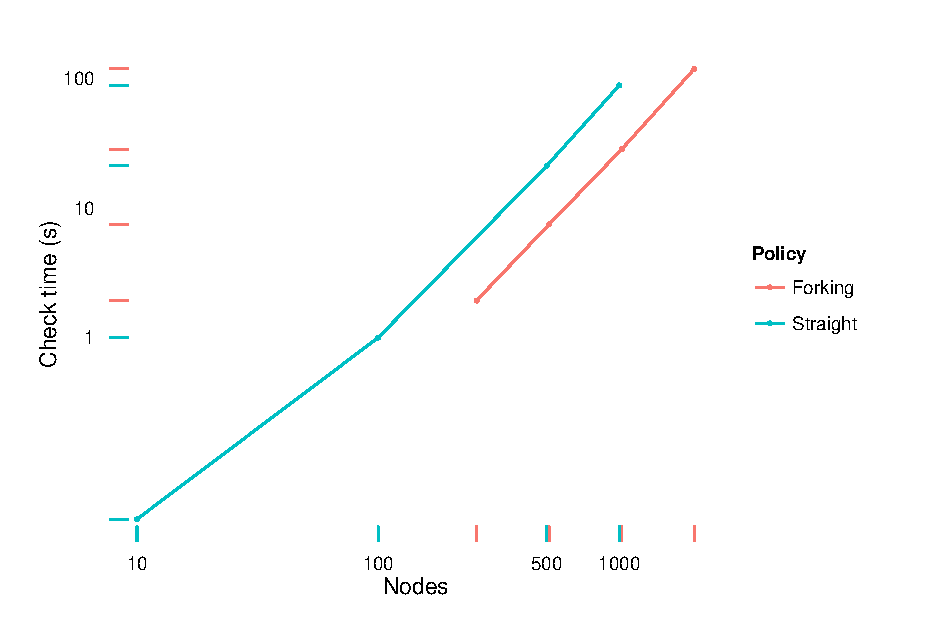
\includegraphics[width=\linewidth]{./images/benchmarks.eps}
  \end{minipage}
  \caption{Bench-marking results on a Nexus 4 Android phone.}
  \label{fig:benchmarks}
\end{figure}

The library has been integrated into a proof-of-concept policy checking app that scans installed apps against four user privacy policies (\autoref{fig:checker}).
This may be extended into something more comprehensive, or into a more polished demo to help promote my research.

\begin{figure}[]
  \centering
  \includegraphics[width=0.5\linewidth]{images/apppal-checker.png}
  \caption{Screen shot from AppPAL checking app.}
  \label{fig:checker}
\end{figure}

\subsection{Explicit policies in stores}

With a means of enforcing policies I wanted to look at the policies already being enforced by the marketplaces.
One source of these policies is in the user and developer agreements required to use or sell apps in the stores.
These policies should give us a good idea about how the stores are used as they are explicit contracts between users, developers and the stores themselves.
We might also be able to describe the differences between stores using AppPAL, to help users pick a store that meets their own policies.

There are many Android app stores available.
I believed that each of the different stores would have different policies for users and developers, and with different privacy conditions.
I read the privacy, developer and user policies for four different app stores (Google Play, Amazon, Aptoide and Yandex) to compare them.
In practice I found that the policies tended to be very similar; perhaps even copied in some places.
There were some differences when it came to payment processing, and minimum ages to use the store.

Some stores (excepting Google's) kept rights to modify any apps, typically for advertising.
This might form the basis of interesting trust relationships.
To install an app Android requires its code is signed by a developer.
Modifying an app would mean the signature is invalid and so the app would need to be re-signed by the store to be installed.
Re-signing is interesting because the trust in the authenticity of the app moves from the developer to the store.

A summary of the different terms and conditions is in \autoref{tab:terms}.

This work could be extended to help users pick an app store that is right for them using a policy.
Projects like COAT~\citep{Fernandez:5lFoplRA} aim to help users pick a store based on their privacy requirements.
We could imagine a similar scheme where AppPAL helps developers decide which stores to submit their apps to,
  and which stores users should buy from.
For example a developer may only agree to sell their app on a store if the store lets them set their own price and they get a 75\% cut of the profits.
\begin{lstlisting}
`dev' says `selling-policy' isMetBy(Store)
  if `dev' setsPriceIn(Store),
     Cut isCutIn(Store).
  where Cut > 0.75.
\end{lstlisting}
\autoref{tab:terms} could be translated into AppPAL and queried to decide which stores can sell the apps; and with this policy only Aptoide would be acceptable.

In Europe and America the choice of which market to use is less interesting.
Only Google's Play store (and to a lesser extent Amazon's app store) has enough market share to be compelling.
In China, however, where the Play store is banned by the government, there is a greater choice of marketplace and this becomes a more compelling avenue of research.

\begin{figure}[!h]\tiny
\begin{tabulary}{\linewidth}{lLLLL}
\toprule
                     & Google Play
                     & Amazon
                     & Yandex
                     & Aptoide \\ \midrule
User ID              & Name address and billing details.
                     & Amazon ID.
                     & None for free apps, payment details for paid.
                     & Contact details. No verification but agreement not to lie.                                                                                                        \\ \addlinespace
Client info taken    & Installation data, device ID, browsing history, cookies. Can opt out.
                     & Device ID, network info, location, usage data.
                     & Device ID, SIM number, Device content, System data, browsing history.
                     & Transaction history.  They may share it with developers.                                                                                                          \\ \addlinespace
Customer Payments    & Google Wallet and others at Google's discretion.
                     & Amazon.
                     & Approved processor by Yandex or store operator.
                     & Approved processor by Aptoide.                                                                                                                                    \\ \addlinespace
Who is paid?         & Google Commerce.
                     & Amazon.
                     & Developer.
                     & Store owner.                                                                                                                                                      \\ \addlinespace
Prices set by        & Developer.
                     & Amazon.
                     & Developer (but Yandex may restrict to set values).
                     & Developer and store owner.                                                                                                                                        \\ \addlinespace
Refunds              & Only for defective or removed content. A refund may be requested for two hours after purchase.
                     & No.
                     & Up to 15 minutes after purchase. No for IAP.
                     & Up to 24 hours after purchase.                                                                                                                                     \\ \addlinespace
Age of use           & At least 13.
                     & Any age (with consent of guardian).  No alcohol related content below 21.
                     & At least 14.
                     & A legal age to form a contract with Aptoide.                                                                                                                      \\ \addlinespace
Update provision     & You agree to receive updates.
                     & By default.
                     & Yes for security and bug-fixes.
                     & Yes agree to receive updates.                                                                                                                                     \\ \addlinespace
Moderation           & No obligation (but they may).
                     & Publisher obliged to provide info which may be used to give ratings.  Amazon will not check these ratings are accurate.
                     & No obligation (but they may).
                     & No obligation (but they may).  Trusted app mark does not indicate moderation.                                                                                     \\ \addlinespace
Acceptable use       & No use as part of a public performance, or for dangerous activities where failure may lead to death.
                     &
                     &
                     & No modification, rental, distribution or derivative works.  You may use the software.                                                                             \\ \addlinespace
Store rights to app  & Marketing and optimising Android.
                     & Distribution, evaluation, modification, advertising, and creating derivatives for promotion.
                     & Advertising.
                     & Modification and re-selling.                                                                                                                                      \\ \addlinespace
Withdrawal from sale & Immediate.
                     & 10 days, or 5 days if for copy-write reasons.
                     & 90 days. A copy will be retained.
                     & You may.                                                                                                                                                          \\ \addlinespace
Developer ID         & Google account and billing details.
                     & Amazon ID.
                     & Email, company name, tax-id.
                     & Email (preferably a Google developer one).                                                                                                                        \\ \addlinespace
EULA                 & Default offered.
                     & Only if it doesn't interfere with Amazon's terms.
                     & Must be provided.
                     & Default offered                                                                                                                                                   \\ \addlinespace
Content restrictions & No alternate stores, sexual, violence, IP infringing, PII publishing, illegal, gambling, malware, self-modifying or system modifying content.  No unpredictable network use.
                     & No offensive, pornography, illegal, IP infringing or gambling content.
                     & No defects. No illegal, disruptive, sexual, IP infringing, PII stealing, alternative stores, or open-source content.
                     & No displaying or linking to illegal, privacy interfering, violent, PII stealing, IP infringing content.  Nothing \emph{spammy} or with unpredictable network use. \\ \addlinespace
Payout rates         & 70\% of the user's payment.
                     & 70\% list price (minus card fees).
                     & 70\% net-revenue (minus card fees).
                     & 75\% revenue share (minus card fees).                                                                                                                             \\ \addlinespace
\bottomrule
\end{tabulary}
\caption{Summary of conditions in different stores.}
\label{tab:terms}
\end{figure}

\subsection{Distribution mechanisms in app stores.}

Whilst the user and developer agreements describe what the apps stores say they will do; to see what they do in practice we need reverse engineering.
A user buying an app probably wants it sent to their device.
Using an SSL proxy I started looking at the distribution mechanisms, and started reverse engineering their protocols.
For simple website stores, such as Opera's mobile store, where apps are distributed without encryption it is trivial to modify downloaded apps on the fly.
A \ac{MITM} attack using a tool like \texttt{mitmproxy} can modify the apps as they are downloaded.
In these stores there was no verification that the app downloaded matched the app requested.

Some issues were found in other stores.
Amazon's store was the only one to enable certificate pinning.
Certificate pinning can prevent SSL sniffing attacks as it requires that the SSL certificate is one known to the app; rather than one that exists in the device's root of trust.
The only pinned certificate, however, was for accessing the login server.
Once the login token had been issued, however, the traffic between the store and the device could be intercepted and decrypted freely.
This isn't a vulnerability as there were other mechanisms in place within the store to prevent app modification: namely cryptographic signatures that came with every app.
It does hint, however, that the login system and the store itself have different security guarantees, which may lead to other problems within the store.

Google's Play Store seemed to sometimes drop encryption when downloading APK files.
To download an app from the store the user has to follow a protocol, which we describe abstractly in \autoref{fig:protocol}.
This was inferred by looking at the network traffic and reverse-engineering the store's APK file.
After completing the purchase the user presents their proof-of-purchase token to the store along with a description of the app and their own ID (messages 5 \& 6)
The store then tells them a server to speak to which provides the app to them without further information (the blank message 7 and message 8).
This is implemented using a URL redirect, where $S$ and $S^\prime$ represent the servers the client talks to.
What we observed, however, is that occasionally the redirect was to a server using HTTP rather than HTTPS.
This meant that an attacker sniffing the traffic could see which apps were being downloaded and take a copy for themselves.
If the sniffing party was an employer, and usage of the app gave away personal information (say a diabetes app or Grindr), then this could be problematic.
By replaying message seven the user (or a third-party who knew the URL) could re-download the app for up to a week later.

Each of the stores I looked at had a slightly different protocol for buying apps and a different means of downloading them onto the device.
In an AppPAL-enhanced app store we might imagine apps being supplied with some assertions about their behaviour.

One way to implement this would be for the store, as part of the download, give the user a bundle of AppPAL statements.
The user could filter these to find the statements that are useful for deciding any policies they may have.
This force the mobile device to do extra processing which is undesirable if running on batteries.
Working out how to send the AppPAL statements in the download protocols, (and with knowledge distribution in general, proposed in \autoref{ssec:kdp}) seems interesting.

\begin{figure}[!h]
  \begin{minipage}{0.48\linewidth}
    \begin{center}
    \begin{tabular}{rrc}
      \toprule
      1. & $C \longrightarrow S$:        & $U, C, a_{\text{d}} $  \\ \addlinespace
      2. & $S \longrightarrow C$:        & $a_{\text{d}}, ? $     \\ \addlinespace
      3. & $C \longrightarrow S$:        & $U, ! $                \\ \addlinespace
      4. & $S \longrightarrow C$:        & $a_{\text{d}}, \$ $    \\ \addlinespace
      5. & $C \longrightarrow S$:        & $U, a_{\text{d}}, \$ $ \\ \addlinespace
      6. & $S \longrightarrow C$:        & $S^\prime$             \\ \addlinespace
      7. & $C \longrightarrow S^\prime$: &                        \\ \addlinespace
      8. & $S^\prime \longrightarrow C$: & $a$                    \\
      \bottomrule
    \end{tabular}
  \end{center}

    {\footnotesize In message 6, $S$ redirects $C$ using a 302-redirect message.
      By replaying message 7 I found I could re-download the app on a different client.
      I found that the redirection to the other server sometimes did not use SSL.}
  \end{minipage}
  \begin{minipage}{0.48\linewidth}
    \begin{tabulary}{\linewidth}{cC}
      \toprule
      Symbol         & Meaning                                                           \\
      \midrule
      $S$            & Store (\texttt{android.clients.google.com}).                      \\
      $C$            & Client the app store app running on the phone.                    \\
      $U$            & User, identified by a token.                                      \\
      $a$            & An app.                                                           \\
      $a_{\text{d}}$ & a description of the app $a$.                                     \\
      $?$            & Purchase challenge                                                \\
      $!$            & Purchase challenge response (seemingly derived from $?$ and $U$). \\
      $\$$           & Download token.                                                   \\
      $S^\prime$     & Alternate store URL                                               \\
      \bottomrule
    \end{tabulary}
  \end{minipage}
  \caption{Abstraction of the protocol used by Google's Play store to purchase an app.}
  \label{fig:protocol}
\end{figure}

\subsection{User app installation behaviour}

Having explored the policies and protocols in the stores we also wanted to explore how the stores are used in practice.
Users have policies about what data apps should be collecting.
Lin~\etal~\citep{Sadeh:2014vq} identified four different user-privacy policies; however they did not look at whether they enforced them in practice.
Using AppPAL I implemented a simplification of the policies Lin~\etal~identified.
The Carat project~\citep{Oliner:2013ht} collected app installation data from users who installed their energy tracking app.
They shared this data with us in an anonymised form where I could see who had installed what; provided I knew the package names of the apps they installed.
Using the \ac{SKB} I de-anonymised 4,300 apps (5\%) which accounted for 50\% of all app installs.
I selected 44,000 users for whom I knew 20 or more app installs.

With the Carat data I measured the extent each user conformed to the privacy policies.
I also took a list of known malware and \acp{PUP} from McAfee to measure the extent of malware installations on Android.
I tested whether users who enforce their privacy policies install less malware.

I found that very few users follow a privacy policy all the time~\citep{Hallett:2015ty}.
A few users, however, seem to be installing apps meeting a policy most of the time.
For the unconcerned policy (the most permissive) only 1,606 users (4\%) had 50\% compliance;
and only 120 users (0.3\%) had 80\% compliance.
For the stricter conservative policy only 60 users were complying half the time, and just 7 users more than 80\% of the time.
This suggests that while users may have privacy preferences the majority are not attempting to enforce them.

I found 1\% of the users had a PUP or malicious app installed.
A user is three times more likely to have a PUP installed than malware.
Only nine users had both a PUP and malware installed.
Users who were complying more than half the time with the conservative or advanced policies complied with the malware or PUP policies fully.
This is significant (P-value $< 0.05$) and suggests that users who pick their apps carefully are less likely to experience malware.

% \begin{figure}\centering
%   \begin{subfigure}[b]{0.48\linewidth}
%     \includegraphics[width=\linewidth]{./images/lin-2yr.eps}
%     \caption{User conformance to identified privacy policies.}
%     \label{s}
%   \end{subfigure}
%   \begin{subfigure}[b]{0.48\linewidth}
%     \includegraphics[width=\linewidth]{./images/malware-2yr.eps}
%     \caption{User malware installation rates.}
%     \label{sfig:malware}
%   \end{subfigure}
%
%   \begin{subfigure}[b]{\linewidth}
%     \includegraphics[width=\linewidth]{./images/compare-2yr.eps}
%     \caption{Comparison of users following the advanced policy with malware installation.}
%     \label{sfig:compare}
%   \end{subfigure}
%
%   \caption{Results from study on user app installation behaviour.}
%   \label{fig:lin}
% \end{figure}

This work was presented as a poster at SOUPS~\citep{Hallett:2015ty}, and I am aiming to publish it as part of a paper targeting the ESSoS conference (a draft of which is attached in the appendix).

\section{Suggested topics for next year}
\label{sec:futurework}

In the thesis proposal I suggested that in the third year I might look at advanced kinds of policies.
I also wanted to look at what might happen when policies have to deal with updates, to the policies and the apps on the device.
Some topics included:
\begin{itemize}
  \item The app collusion problem.
  \item What happens when policies are composed?
  \item Policy revocation and modification.
  \item App update policies.
\end{itemize}

Some of these problems have become less interesting: for example app updates.
Various different policies could be encoded in AppPAL for the precise behaviour of an update.
Since most stores mandate accepting updates in the user agreement, and the default behaviour is to auto-install updates, these schemes are unrealistic.
Updates typically include bug-fixes so it is in the user's interests to accept them (despite what they may believe~\citep{Vaniea:2014fk}).
Implementing methods to weaken security does not seem to be worthwhile.
Using AppPAL as a modelling language to precisely describe the trust mechanisms and delegations in an update is interesting.
It might make sense to include a comparison of the different update mechanisms in Android and iOS in the thesis.

Policy modification is less interesting.
Apps should be rechecked before they can be allowed to run again.
If they now break the policy, the user should be prompted to remove the app or make an exception.
Results from long-running analysis tools can be stored by the \ac{SKB}.
These could be reused by AppPAL's constraint mechanisms to avoid re-computation, if no other changes were made.

The app collusion problem is interesting.
Whilst it is conceivable that AppPAL policies could describe and prevent attacks, to actually implement the protection in a way that could be used would probably require modifications to the intent system, and potentially binder (Android's primary IPC mechanism).
This probably makes it out of scope of the PhD as we are looking at Android, not a modification of it.

The mechanisms for mechanically composing policies in AppPAL are trivial\footnote{\lstinline{`user' says `composed-policy' isMetBy(App)  if `pol1' isMetBy(App), `pol2' isMetBy(App).}} but what might happen when two principals actively disagree is more interesting.
AppPAL doesn't have support for negation, but it feels right that there should be some way to distinguish between a principal saying an app meets, does not meet, or does not know whether it meets a policy.
Work next year should look at the protocols for distributing AppPAL statements.

\subsection{Knowledge distribution protocol}
\label{ssec:kdp}

AppPAL can enforce policies and I have started looking at the kinds of policies users might want to use.
When describing AppPAL policies I have thought about delegation relationships and how different principals can be trusted to help make decisions.
What isn't necessarily clear is how these principals get to make these statements and how they are transferred from speaker to speaker.

On a memory constrained device, like a mobile phone, storing a database of all possible AppPAL statements by every speaker is not viable.
There are almost 1.5 million apps available on the Google Play store not including other stores or multiple versions of the same app.
Storing data on all apps will not work as the file size will be huge.
In the papers on SecPAL~\citep{Becker:2006vh,Becker:2009vt} (on which AppPAL is based) there is little talk about how the knowledge should be distributed.
\citeauthor*{Becker:2006vh} describe how principals should sign their AppPAL statements to identify themselves as having said them, and how an X.509-style public key system could be used to tie keys to principals.
This tells us how to check the statements are not forged but does not give the distribution mechanisms.
Related languages~\citep{Becker:2009ula,Aziz:2011vt,Gurevich:2008fz,Gurevich:Qo5E3M3} extended SecPAL features but still didn't specify the distribution protocol.
SecPAL was built to be a distributed language with principals delegating statements.
Without a distribution protocols some scenarios can become difficult.

Consider Alice who wants to install an app on her phone.
Her installation policy requires confirmation the app is not malware.
She knows that McAfee can say (possibly with further delegation) whether an app is malicious or not;
  but this is a new app and she does not have any prior information about it.
She needs to get more information.

One, very simple, approach to distribute the knowledge might be to use a protocol such as:
\begin{center}
  \begin{tabular}{rrc}
    \toprule
    1. & $U \longrightarrow S$:        & $q, d?, m$ \\ \addlinespace
    2. & $S \longrightarrow U$:        & $r, t,  \left\{ r, t \right\}_{S_{SK}}$  \\ \addlinespace
    \bottomrule
  \end{tabular}
\end{center}
A user ($U$) wishes to find out if a server ($S$) knows any information that will help them answer a query ($q$).
To do this they send the server the query along with any metadata they have, for example the app itself, to the server and say whether they'll allow the server to delegate ($d?$).
In reply the server sends any information it thinks would be helpful ($r$), plus a timestamp ($t$) and a signature on the response and timestamp so the user is sure they're receiving fresh information.
If the user finds they need more information then the protocol will need to be replayed.

This gives a simple protocol for distributing knowledge but it doesn't deal with all the complexities of knowledge distribution.
In particular:
\begin{itemize}
  % \item
  %   How does she ask McAfee about the app?
  %   What is the protocol for speaking and distributing statements?
  \item
    If the app is new McAfee may not know about it either.
    How should she send it to them for analysis?
    In the protocol we suggested the app itself could be sent as part of the metadata relating to the query.
    There may be legal issues surrounding Alice redistributing the app to McAfee, however.
    If the app is large and Alice has a limited data-allowance she may not want to send the whole app.
    She could just send a link to the app on an app store, but McAfee may not want to check it if it costs money to download, or the terms of buying the app prevent reverse engineering.
  \item
    How do McAfee respond when they can't answer the query?
    AppPAL does not contain negation but in this scenario it would be helpful to distinguish a statement from McAfee that the app is safe, from one where they know it is definitely malware, from one where they are unsure and wish to err on the side of caution and not make a definite statement.

  \item
    What should Alice do while she waits: keep waiting, fail and keep a note to recheck later or fail and never ask again about the app?
    Should she say how long she is willing to wait so McAfee can distinguish between needing an answer now (Alice is trying to use the app right now) or that the answer isn't urgent (her phone is caching information about apps she hasn't bought yet in case she buys one of them in the future).
  \item
    If McAfee wish to delegate the decision they could issue another \emph{can-say} statement.
    Should McAfee send the public key and any statements from the delegated party to the user, or just the server address and a reference to the public key on a PKI server?
  \item
    When should Alice ask McAfee?
    Before any evaluation would be the easiest time as it would require no change to the evaluation algorithm but during the evaluation might be more appropriate as statements could be imported as needed.
\end{itemize}

Work this year should look at developing a strategy, and defining a protocol to share and acquire knowledge through AppPAL statements on demand.
This would be a worthwhile contribution, as it is novel, and would help extend AppPAL from a SecPAL instantiation to its own language.
To do this we aim to complete the following goals:
\begin{itemize}
  \item
    Define a protocol where a principal can query another principal for information.
    The protocol must define precisely what should happen when a further delegation occurs.
  \item
    Show that AppPAL (or SecPAL) is still sound and complete when using this protocol as part of its evaluation.
  \item
    Integrate the protocol with the AppPAL library and check the performance impact from using it.
    Explore different strategies for what to do while waiting for answers, and how AppPAL could be configured to switch between them.
  \item
    Demonstrate use of the protocol using the \ac{SKB} as a third-party who can be queried for information.
\end{itemize}

\subsection{Case study}

Having an authorization logic model and enforce a larger, currently implemented policy shows the limitations and expressivity of a language.
It also shows that it is applicable to current compliance problems and is more than just a toy.
AppPAL policies I have used so far have been synthetic.
This has been fine for testing and demonstrating the language, but a larger example drawn from a real security policy would help give AppPAL credibility.

A natural source for this policy is a corporate \ac{BYOD} policy where employers restrict the usage of mobile devices in the workplace.
The \ac{NIST} have published recommendations for mobile device security and \ac{BYOD} in the workplace~\citep{Souppaya:2013jf,Scarfone:2009vy}.
Translating the recommendations into AppPAL and showing their enforcement would make a good case study.
The study would focus on any difficulties in translating the policies and the extent the recommendations could be enforced automatically.
Specifically we would aim to:
\begin{itemize}
  \item
    Present an AppPAL policy derived from the guidelines in Sections 2--3 of NIST-SP-800-46 (which gives guidelines for telework and remote access mobile security) and Section 2 of NIST-SP-800-124 (guidelines for mobile security).
  \item
    Show where the strengths and limits of AppPAL lie when enforcing the guidelines.
  \item
    It is reasonable to expect that we cannot automatically enforce every aspect of the guidelines as they are high level and written in natural language.
    Some aspects of the guidelines will need a human to certify that it is met.
    Using AppPAL we can show where a human will be needed and measure the extend of automatic enforcement.
\end{itemize}

\section{Plan for thesis submission}

\begin{quote}
  \emph{Hypothesis.} Automatic tools and policy languages would provide a
  better means of enforcement for mobile device policies than existing
  mechanisms which rely on manual inspection.
\end{quote}

I have 18 months remaining, with my funding running out in March 2017.
My plans for the time remaining are shown in \autoref{fig:gantt}.
The next year will be primarily spent completing the projects described in \autoref{sec:futurework}; and continuing any other work that seems interesting as opportunities arise.
Once my review is completed I plan to spend at least one day a week writing up work for my thesis; focussing on the literature review, and completed investigations.
From October 2016 I plan to spend the majority of my time writing (as suggested in my thesis proposal).
From January 2017 I plan to be predominantly focusing on editing.
I believe this is a reasonable plan based on my writing speed, and the time I typically spend editing documents.

\begin{figure}
\caption{Gantt chart showing plan for time remaining.}
\includegraphics[width=\linewidth]{gantt.pdf}
\label{fig:gantt}
\end{figure}

Below is a proposed table of contents for the thesis, with content suggestions for each chapter.
\begin{enumerate}
  \item Introduction
  \item Mobile ecosystems
    \begin{description}
      \item[App stores and mobile app deployment]
        \hfill
        \begin{itemize}
          \item Introduce app stores and current development practices.
          \item Show the differences between different market places and the platforms (iOS vs Android).
        \end{itemize}
      \item[Android Security Model]
        \hfill
        \begin{itemize}
          \item Give overview of Android security architecture.
          \item Describe how apps work and interact with the system from a technical perspective.
          \item Introduce the android permissions model and how different apps can access functionality provided by the platform.
          \item Show how app signing works.
        \end{itemize}
      \item[Android policies]
        \hfill
        \begin{itemize}
          \item Introduce the need for policies and the motivation for the PhD.
          \item Show how users do not seem to be following their privacy policies.
          \item Explain how some companies have mobile device policies, and how users are frustrated with data leaks.
          \item Show existing tools, such as Kirin, and explain why they're not good enough.
        \end{itemize}
    \end{description}
  \item AppPAL Implementation
    \begin{description}
      \item[The need for a policy language]
        \hfill
        \begin{itemize}
          \item Introduce scenarios where AppPAL can be used to enforce a policy
          \item Show trust relationships between different principals (a user at work).
          \item Start to introduce the language.
        \end{itemize}
      \item[Design and implementation of AppPAL]
        \hfill
        \begin{itemize}
          \item Formally present the language, as an instantiation of SecPAL.
          \item Show evaluation algorithm.
        \end{itemize}
    \end{description}
  \item AppPAL Experimentation
    \begin{description}
      \item[Deployment]
        \hfill
        \begin{itemize}
          \item Show applications using AppPAL.
          \item Stores generated by policy.
          \item On device policy checking.
          \item Device configuration by policy (if I can get access to Android M features)
        \end{itemize}
      \item[Distribution]
        \hfill
        \begin{itemize}
          \item Define protocol for knowledge acquisition.
          \item Describe implementation of protocol.
          \item Implement the protocol as part of AppPAL's evaluation algorithm.
        \end{itemize}
    \end{description}
  \item Evaluation
    \begin{description}
      \item[User privacy policies]
        \hfill
        \begin{itemize}
          \item Show privacy paradox with Android apps.
          \item Use Carat (and McAfee?) data as a model of what users have installed.
          \item Show power of AppPAL as a query and modelling language.
          \item Discuss the policies users do seem to be enforcing in practice.
        \end{itemize}
      \item[Case study]
        \hfill
        \begin{itemize}
          \item Present \ac{NIST} guidelines for mobile device guidelines for managing the security of mobile devices in the enterprise expressed in AppPAL.
          \item Show the language is expressive enough to describe enterprise policies.
          \item Discuss problems translating the recommendations, and where the guidelines could not be checked without manual intervention.
        \end{itemize}
    \end{description}
  \item Related work
  \item Future work
\end{enumerate}

\bibliography{report}

\newpage
\appendix

\section{Paper for ESSoS 2016}

The attached paper is a draft being prepared for the ESSoS\footnote{Engineering Secure Software and Systems} symposium.
The paper will introduce the AppPAL language and its implementation.
I give sanity checking benchmarks to show its performance is not unreasonable.
Finally, I demonstrate AppPAL by presenting our work using AppPAL to filter user's privacy policies from our SOUPS poster, as part of a full paper.

\newgeometry{left=0.01em,top=0.01em, right=0.01em, bottom=0.01em}
\includepdf[pages=-]{../essos-2016-apppal/paper.pdf}

\end{document}

